\documentclass[sigconf]{acmart}
\usepackage{graphicx}
\graphicspath{ {images/} }

\usepackage{booktabs} % For formal tables

\begin{document}
\title{Determining Predictors of H-1B Salary and Approval}
\subtitle{Milestone Report}


\author{Wenhao Yu}
\affiliation{%
  \institution{University of Notre Dame}
  \city{South Bend}
  \state{Indiana}
}
\email{wyu1@nd.edu}

\author{Luke Duane}
\affiliation{%
  \institution{University of Notre Dame}
  \city{South Bend}
  \state{Indiana}
}
\email{lduane@nd.edu}

\author{Will Badart}
\affiliation{%
  \institution{University of Notre Dame}
  \city{South Bend}
  \state{Indiana}
}
\email{wbadart@nd.edu}


\begin{abstract}
The paper presents the findings of the H-1B visa program analysis project for CSE-40647/60647.
The project sought to determine which features of an H-1B application were the strongest predictors
of that application's certification status\footnote{A {\it certified} visa is valid for further
processing, while an {\it approved} enables the holder to live and work in the country.}.
\end{abstract}

\maketitle


\section{Introduction}

The H-1B visa program, enacted by the Immigration and Nationality Act of 1965, opens the door for
immigrants in specialized professions to migrate to the United States for an extendable term of up to six
years \cite{FederalRegister}. Last year, in 2017, almost 350,000 foreign workers applied for the program,
and just under 200,000 were approved \cite{DHS}.

All H-1B visas are sponsored by the hiring organization (i.e. future employer of the immigrant).
The organization creates an application for each foreign worker it intends to hire and submits them to
the Department of Labor for certification.
Certified applications are subsequently submitted to the annual H-1B lottery, the process which
determines which of the many certified applications are actually approved \cite{USCIS}.

The H-1B application pipeline is a laborious and complex process for {\em both} large companies bringing
in thousands of migrant employees and small ones onboarding only a couple. A tool which
highlights the important features that support H-1B approvals could be a vital strategic asset for
these companies. Lots of data exists in this domain, but to integrate it and perform meaningful
analysis is beyond the capabilities of companies without established data science practices.
We plan to produce a model that shows what features are most valuable in regards to H-1B application
certification.

A related analysis with tangible business value would model worker salaries as a function of other
application attributes, allowing companies to optimize wages for their H-1B employees against those
other attributes.


\section{Related Work}

In April of 2017, Glassdoor published an article analyzing the salaries of H-1B immigrants and
comparing them to those of domestic workers in similar roles and fields. While the report does
not attempt to model H-1B workers' salaries based on other features, it offers a comprehensive
statistical analysis of their pay \cite{Glassdoor}.

We were unable to find any prior investigation attempting to model H-1B visa certification
against public application attributes.


\section{Problem Definition}

How can we predict the approval status of a given H-1B via certification? What tangential
analyses provide tangible business value for companies sponsoring H-1B visas? How would the salary
range change based on a given occupation?


\section{Methodology}

The sheer volume of data available to train our model (over three million records) necessitated
that we perform a number of initial analyses before constructing the models. For these initial
analyses, we chose to calculate a number of descriptive statistics over our primary data set\footnote{See
\ref{subsec:datasets} Datasets} as well as a couple visualizations to quickly understand the
distributions of key features.
We have already identified a few outliers in the primary dataset (in particular, in the
$PREVAILING\_WAGE$ feature) and cleaned our data before producing our initial findings. The
cleaning process simply drops rows with extreme values.

The baseline is a Naive Bayes model which looks at a configurable subset of features to predict
an unseen application's certification status. This model (as well as all of our more advanced models)
is trained on 75\% of the available data and tested on the remaining 25\% of records.

For the project, we created an extensible classification framework which allowed us to test
various models with different parameterizations over the same train/ test partitionings. The other
models we experimented with were decision trees (both ID3 and CART, each tested with all available
branching strategies), and a multi-layer perceptron (tested with different hidden-layer sizes,
activation functions, and solvers)\footnote{See \ref{sec:experiments} Data and Experiments}.

\subsection{Feature Engineering}

The primary dataset contains over 200,000 different job titles (i.e. values of the $JOB\_TITLE$
feature). We anticipated that using this feature in its raw state would hurt decision tree
performance (at least for ID3) due to its highly branching nature.

Therefore, we engineered the $JOB\_CLUSTER$ categorical feature, which has only eight values
(we created 8 clusters). The raw strings which populated the $JOB\_TITLE$ column were unsuitable
inputs to any clustering algorithm, so we first used a {\it count vectorization} strategy to
turn each string into a vector. The length of the vector is equal to the size of the vocabulary
(the number of unique words from {\it all} job titles); each element corresponds to one word in
the vocabulary and the value at that index holds the number of times that word occurred in the
job title (almost always $1$).

Once the set of job titles was tokenized and transformed into a sparse matrix as described above,
we were able to cluster the job titles with a couple different algorithms and parameterizations.
We heuristically determined that \texttt{SpectralClustering} with $k = 8$ produced the highest
quality clustering of job titles. This was the model we used to compute the $JOB\_CLUSTER$ feature.


\section{Data and Experiments}
\label{sec:experiments}

\subsection{Datasets}
\label{subsec:datasets}

\begin{enumerate}

\item One of the largest freely available datasets on H-1B applications comes from
\href{https://kaggle.com}{kaggle.com}. It contains over 3 million records and tracks 10 different features
per application\footnote{See \href{https://www.kaggle.com/asavla/h1-visa/data}{kaggle.com/asavla/h1-visa/data}}.
This data covers applications roughly between 2012 and 2016.

\item Another key dataset comes from the Foreign Labor Certification Data Center. Its data is
organized by year, spanning from 2001 to 2007\footnote{See
\href{http://www.flcdatacenter.com/CaseH1B.aspx}{flcdatacenter.com/CaseH1B.aspx}}.

\item OFLC's annual reports also provides a lot of program information and data. Although
it is not raw data, it disclosures cumulative quarterly and annual releases of program to assist
with external research and program evaluation\footnote{See
\href{https://www.foreignlaborcert.doleta.gov/pdf/OFLC_Annual_Report_FY2016.pdf}{https://www.foreignlaborcert.doleta.gov/pdf/OFLC\_Annual\_Report\_FY2016.pdf}}.

\end{enumerate}


\subsection{Data Summary}
This subsection presents a preliminary description of dataset (1), the Kaggle dataset described in
section \ref{subsec:datasets} Datasets.

%% TODO: update this with new description.py output
Figure \ref{fig:salary} shows the salary distribution. There are 5 outliers in the original data.
The average of salary is 72,221, the median of salary is 66,602, and the standard deviation is 24,704.

\begin{figure}[h]
    \caption{Salary Distribution}
    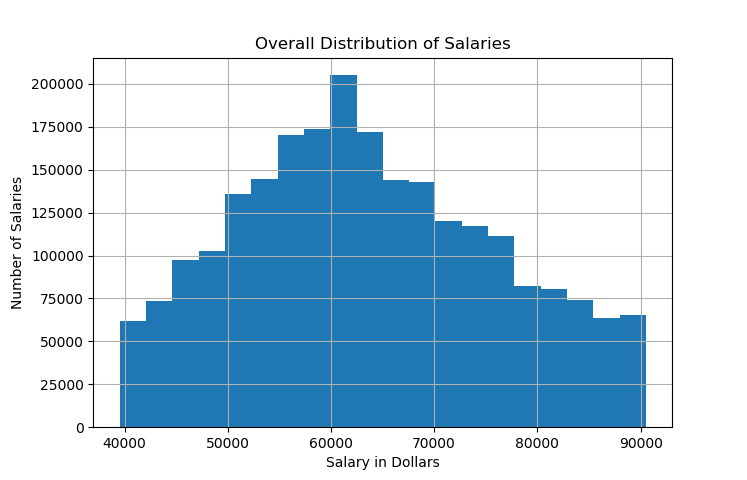
\includegraphics[scale=.4]{salary.png}
    \label{fig:salary}
\end{figure}

Table \ref{tab:classes} shows the frequency of each value of the $CASE\_STATUS$ feature,
the column which labels whether an application was certified. From the dataset's documentation:

\begin{quote}
The $CASE\_STATUS$ field denotes the status of the application after LCA\footnote{Labor Condition
Application} processing. Certified applications are filed with USCIS for H-1B approval.
$CASE\_STATUS = CERTIFIED$ does not mean the applicant got his/her H-1B visa approved, it just
means that he/she is eligible to file an H-1B.
\end{quote}

As demonstrated in Table \ref{tab:classes}, our dataset is characterized by heavy class
imbalance. This lead to special considerations in some of our experiments, such as performing
stratified sampling in the partitioning of testing and training subsets.

This table also shows that most H-1B applications are certified.

\begin{table}[h]
	\caption{Approval Status Classes}
    \begin{tabular}{l l}
        Class Name &Frequency \\
        \hline
        CERTIFIED       & 914,251 \\
        NON-CERTIFIED   & 134,325\\
    \end{tabular}
    \label{tab:classes}
\end{table}

We also chose to examine the change in volume in H-1B applications over time (see Table
\ref{tab:salary}).

\begin{table}[h]
	\caption{Salary Classes}
    \begin{tabular}{l l l}
        Class Name&Frequency&Range \\
        \hline
        Very High   & 90,004   & [104042,E99)\\
        High        & 182,226  & [79331,104042)\\
        Middle      & 361,845  & [59155,79331)\\
        Low         & 181,648  & [28963,59155)\\
        Very Low    & 98,528   & [12584,28963)\\
    \end{tabular}
    \label{tab:salary}
\end{table}

Table 2 shows the frequency of each value of the WAGE feature. We have five categories and the
columns show the frequency and salary range of each class.

\begin{figure}[h]
  \centering
  \includegraphics[width=0.5\textwidth,height=\textheight,keepaspectratio]{byyear}
  \caption{H-1B Application Volume by Year}
\end{figure}


\subsection{Experimental Settings}
About the approval status classification, we use four features: EMPLOYER, JOB TITLE, LOCATION,
SALARY with the label CASE\_STATUS, which has two categories: CERTIFIED and NON-CERTIFIED.

About the salary level classification, we use three features: EMPLOYER, JOB TITLE, LOCATION and the
label is SALARY, which has five categories: VERY HIGH, HIGH, MIDDLE, LOW,VERY LOW.

The clustering task was a bit of a different beast. There were 287,551 different job titles listed
in the primary dataset, so mapping them into the real space to compute and visualize their groupings
was a challenge. The method we decided on first vectorized each job title in a modified one-hot
encoding, turning the set of job titles into a sparse, high-dimensional matrix.

In order to visually evaluate the quality of each clustering, we reduced the dimensionality of our
data matrix down to 2 through $SVD$. We also found that performing the $SVD$ transformation
significantly improved the runtime performace of the $SpectralClustering$ method.

This encoding is compatible with the clustering methods presented by \texttt{scikit-learn}. Figure 3
are the results of clustering with $K$ ranging from 2 to 8.

Each cluster can be characterized by the job title terms that appear most frequently within it. In
general, we found at least one cluster dominated by C-suite officers, another by directors, another
by managers, and sometimes, one by engineering. This provides meaningful groupings of the records
according to job position information.

\begin{figure*}[ht]
  \centering
  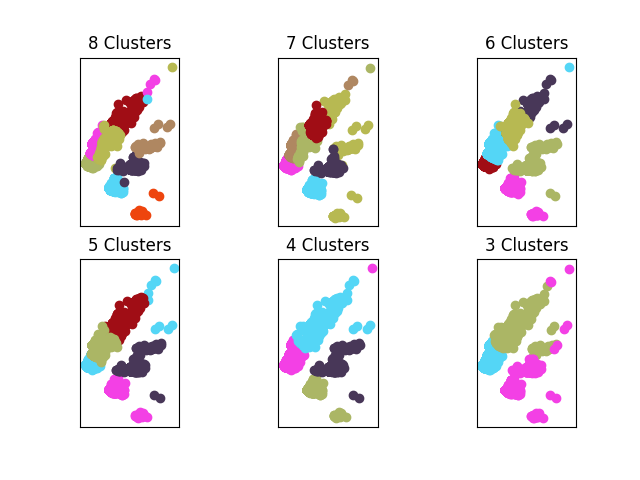
\includegraphics[]{clustering}
  \caption{Clustering on JOB\_TITLE for first 20,000 records (3,433 unique titles)}
\end{figure*}

\subsection{Evaluation Results}

\begin{table}[h]
    \caption{Naive Bayes Confusion Matrix for Approval}
    \centering
    \begin{tabular}{c| c |c}
        &Predicted Approved&Predicted Denied\\
        \hline
        Approved& 888435& 25814\\
        Denied  & 98423 & 35901\\
        %GENTABLE
    \end{tabular}
\end{table}

Accuracy: 0.91409770402 \qquad Specificity:0.26727167


\begin{table}[h]
    \caption{Decision Tree Confusion Matrix for Approval}
    \centering
    \begin{tabular}{c| c |c}
        &Predicted Approved&Predicted Denied\\
        \hline
        Approved& 905932& 8317\\
        Denied  & 81756 & 52568\\
        %GENTABLE
    \end{tabular}
\end{table}

Accuracy: 0.881516343609 \qquad Specificity:0.3913522

\begin{table}[h]
    \caption{Naive Bayes Salary Prediction Accuracy}
    \centering
    \begin{tabular}{l | l | l}
        Class & Correct & Wrong \\
        \hline
         Very High& 58282 &31722 \\
         High     & 93270 &88956 \\
         Middle   & 276983&84862 \\
         Low      & 96456 &85198 \\
         Very Low & 71492 &27063 \\
         \hline
         Total Accuracy & 65.2%
         %GENTABLE
    \end{tabular}
    \label{tab:my_label}
\end{table}

\begin{table}[h]
    \caption{Decision Tree Salary Prediction Accuracy}
    \centering
    \begin{tabular}{l | l | l}
        Class & Correct & Wrong \\
        \hline
         Very High& 67667 &22337 \\
         High     & 137068&45158 \\
         Middle   & 317643&44202 \\
         Low      & 151558&30090 \\
         Very Low & 95306 &3222 \\
         \hline
         Total Accuracy & 84.1%
         %GENTABLE
    \end{tabular}
    \label{tab:my_label}
\end{table}

\section{Conclusions}

\section*{Reference}
[1]  The-Morgan-Kaufmann-Series-in-Data-Management-Systems-Jiawei-Han-Micheline-Kamber-Jian-Pei-Data-Mining.-Concepts-and-Techniques-3rd-Edition-Morgan-Kaufmann-2011-3


\bibliographystyle{ACM-Reference-Format}
\bibliography{main}

\end{document}
